\section{Introduction}
\IEEEPARstart{I}{ndustrial-agent} deployments translate task-level goals into
operations over production signals and equipment. Each operation depends on
the active line, product, recipe, run, and device mapping. A reliable software
path must therefore connect task context to device access and preserve the
sequence from command issue to process response.

Recent work explores end-to-end automation, control-sequence generation,
modular factory skills, and robotic-line control
\cite{xia2025control,huang2026made,koehle2026llmdriven,waseem2026pretrained}.
Other studies address programmable logic controller (PLC) code generation,
context-aware control, resource discovery, shop-floor coordination,
digital-twin fault handling, and natural-language machine access
\cite{liu2026agents4plc,wu2025instructmpc,lim2025llmenabled,zhao2026shopfloor,gill2025llmdt,hofmann2025nlc}.
Recent platforms further connect proposals to Asset Administration Shell
(AAS) models and signed approval, validate actions against process and
instrumentation diagrams (P\&IDs), or organize sensor--manufacturing
execution system (MES)--enterprise resource planning (ERP) evidence streams
\cite{graul2026aas,schall2026safe,lin2026agentic}. Together, these efforts
provide valuable methods for agent reasoning, production context, and
operation constraints.

An integration question remains central to deployment: how should a common
task runtime accommodate different agent engines and direct operation calls,
while translating scene-specific signals into device actions and retaining
the resulting process evidence? AgentWorkShop addresses this question through
a shared operation path. Registered harnesses bind agent engines to task
context; direct REST calls reach the same named-operation dispatcher. Scene
blueprints define semantic signal mappings, targets, and guards, while
configured drivers connect operations to device nodes.

Fig.~\ref{fig:control-path} summarizes this control path. Task goals and
production context inform an operation proposal. Shared checks, route guards,
configured approval, and a pre-dispatch context recheck precede writes through
the device write-control (DCW) subsystem. Command receipts and subsequent
data-acquisition (DAQ) observations remain distinct records, so the software
can relate an issued action to the process response.

\begin{figure}[!b]
\centering
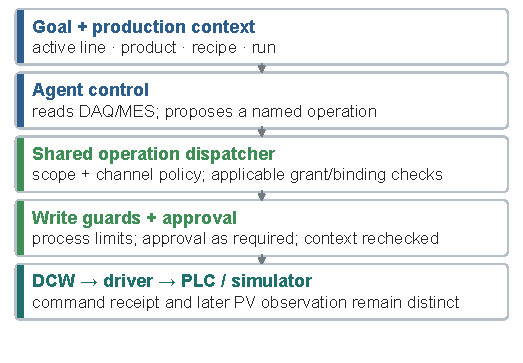
\includegraphics[width=\columnwidth]{resources/fig-agent-control.pdf}
\caption{Agent-control path for a configured industrial task. The agent uses
DAQ and MES context, passes shared operation checks, and routes writes through
process guards, conditional approval, and a pre-dispatch context recheck. DCW
and configured drivers provide device access; command receipts and later
process observations remain separate. Scene configuration supplies targets
and guards, while the application provides its optimization policy.}
\label{fig:control-path}
\end{figure}

AgentWorkShop implements this path as a modular task-to-device framework.
Task and chat requests enter the collaboration runtime, where harness
adapters connect different agent engines to production context, analysis
services, DAQ/DCW nodes, and protocol-specific drivers. Command-line, web,
software development kit (SDK), Representational State Transfer (REST),
Model Context Protocol (MCP), and Agent-to-Agent (A2A) interfaces serve
different callers. Scene blueprints and channel profiles define the available
signals, objectives, guards, tools, and agent bindings. Fig.~\ref{fig:arch}
shows these architectural relationships, and Fig.~\ref{fig:runtime} follows
one registered task through the execution path.

This paper makes two contributions. First, it presents a modular architecture
that coordinates task entry, harness adapters, named operations, shared
checks, configured device access, DAQ/DCW node bindings, and service-owned
evidence. Second, it evaluates the shared execution path through a route study
across four entry paths and two simulator scenes, a mock-state approval-context
test, and a blueprint onboarding replay. A separate archived seed-42 record,
outside that evaluation, illustrates the operation--response--judgment sequence
across four process objectives. The route study checks entry-specific records
and node bindings; the approval test isolates the tuple comparison; and the
onboarding replay instantiates one documented coating line in simulation.

Section~II reviews related work. Section~III presents the design rationale,
architecture, and execution flow. Section~IV explains the core module
functions and their integration. Section~V reports the route study, approval
test, onboarding replay, and archived optimization record. Sections~VI and~VII
interpret the findings and conclude the paper.
